% !TEX root =  ../Dissertation.tex

\chapter{Background}
\label{sec:background}

\section{Reinforcement Learning}
\label{sec:reinforcement_learning}

% Reinforcement Learning (RL) \cite{sutton2018reinforcement} is an artificial intelligence learning paradigm, which, along with supervised and unsupervised learning, constitutes one of the three main approaches in machine learning. What distinguishes RL from other approaches is that the learning occurs through a trial-and-error process, where an \textbf{agent} receives \textbf{reward} signals (positive or negative) from an \textbf{environment}, leading to a focus on maximizing long-term positive rewards. The key elements, the agent and the environment, interact iteratively: the agent observes the state of the environment, takes an action accordingly, and receives a reward along with the next state from the environment (see Figure \ref{fig:rl_loop}). The primary goal of an RL agent is to maximize the cumulative reward, also known as the \textbf{return}. In this section, we will formally define these concepts.

Reinforcement Learning (RL) \cite{sutton2018reinforcement} is one of the three main paradigms in machine learning, alongside supervised and unsupervised learning. What distinguishes RL from other approaches is that the learning involves a trial-and-error process in which an \textbf{agent} interacts with an \textbf{environment} to maximize long-term rewards. The agent iteratively observes the current state of the environment, takes an action, and receives a \textbf{reward} signal (positive or negative), along with the next state (see Figure \ref{fig:rl_loop}). The primary objective of the RL agent is to maximize the cumulative reward, or \textbf{return}. In this section, we will formally define these concepts.

\begin{figure}[H]
    \centering
    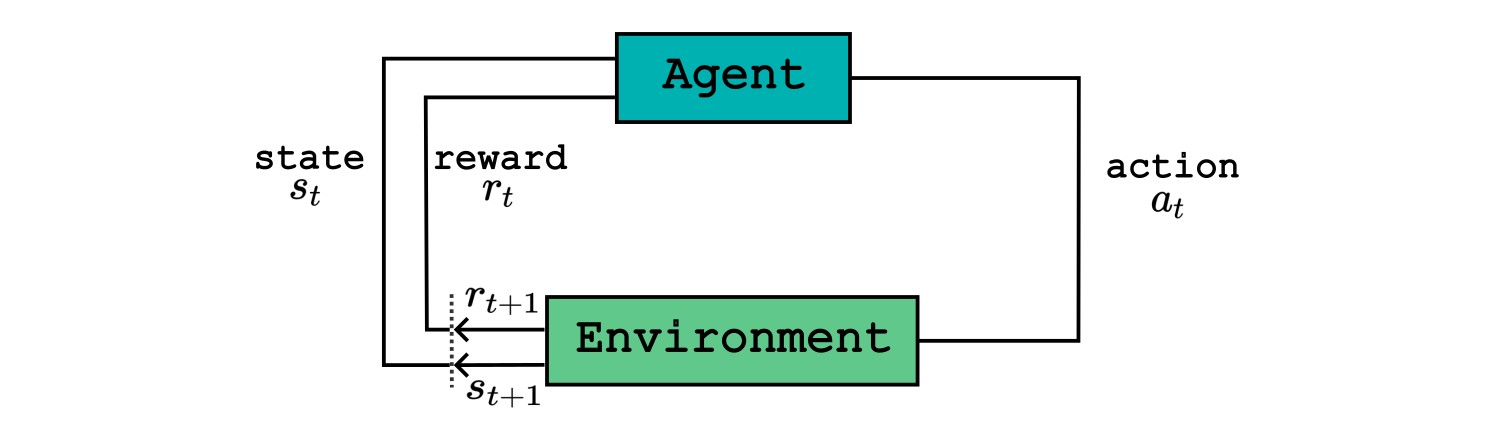
\includegraphics[width=1\linewidth]{Figures/rl_loop.jpg}
    \caption[Reinforcement Learning Loop]{\textbf{Reinforcement Learning Loop.} TODO}
    \label{fig:rl_loop}
\end{figure}

% MDPs
\subsection{Markov Decision Process}
\label{sec:mdp_definition}

\textbf{Markov Decision Processes} (MDP) provide the formal framework upon which most RL algorithms are built. A \textbf{finite} MDP is an state transition system defined as a 5-tuple $M = \langle \mathcal{S}, \mathcal{A}, \mathcal{P}, \mathcal{R}, \gamma \rangle$, where 

\begin{itemize}
    \item $\mathcal{S}$ is a finite set of states,
    \item $\mathcal{A}$ is a finite set of actions,
    \item $P : \mathcal{S} \times \mathcal{A} \rightarrow \mathcal{P(S)}$ is a transition kernel, where $\mathcal{P(S)}$ is the set of probability distributions on $S$, and $P(s'|s, a)$ is the probability of transitioning from state $s$ to state $s'$,
    \item $\mathcal{R} : \mathcal{S} \times \mathcal{A}  \rightarrow \mathbb{R}$ is the reward function,
    \item and $\gamma \in [0, 1)$ is a discount factor.
\end{itemize}

For reference, a MDP can be visualized as a graph, as shown in Figure \ref{fig:mdp}, where the interaction between all components is illustrated. A MDP intuitively could be understood as the environment, while the agent decision-making mechanism is defined by a policy, which induces a Markov Chain on top of a MDP.

\begin{figure}[H]
    \centering
    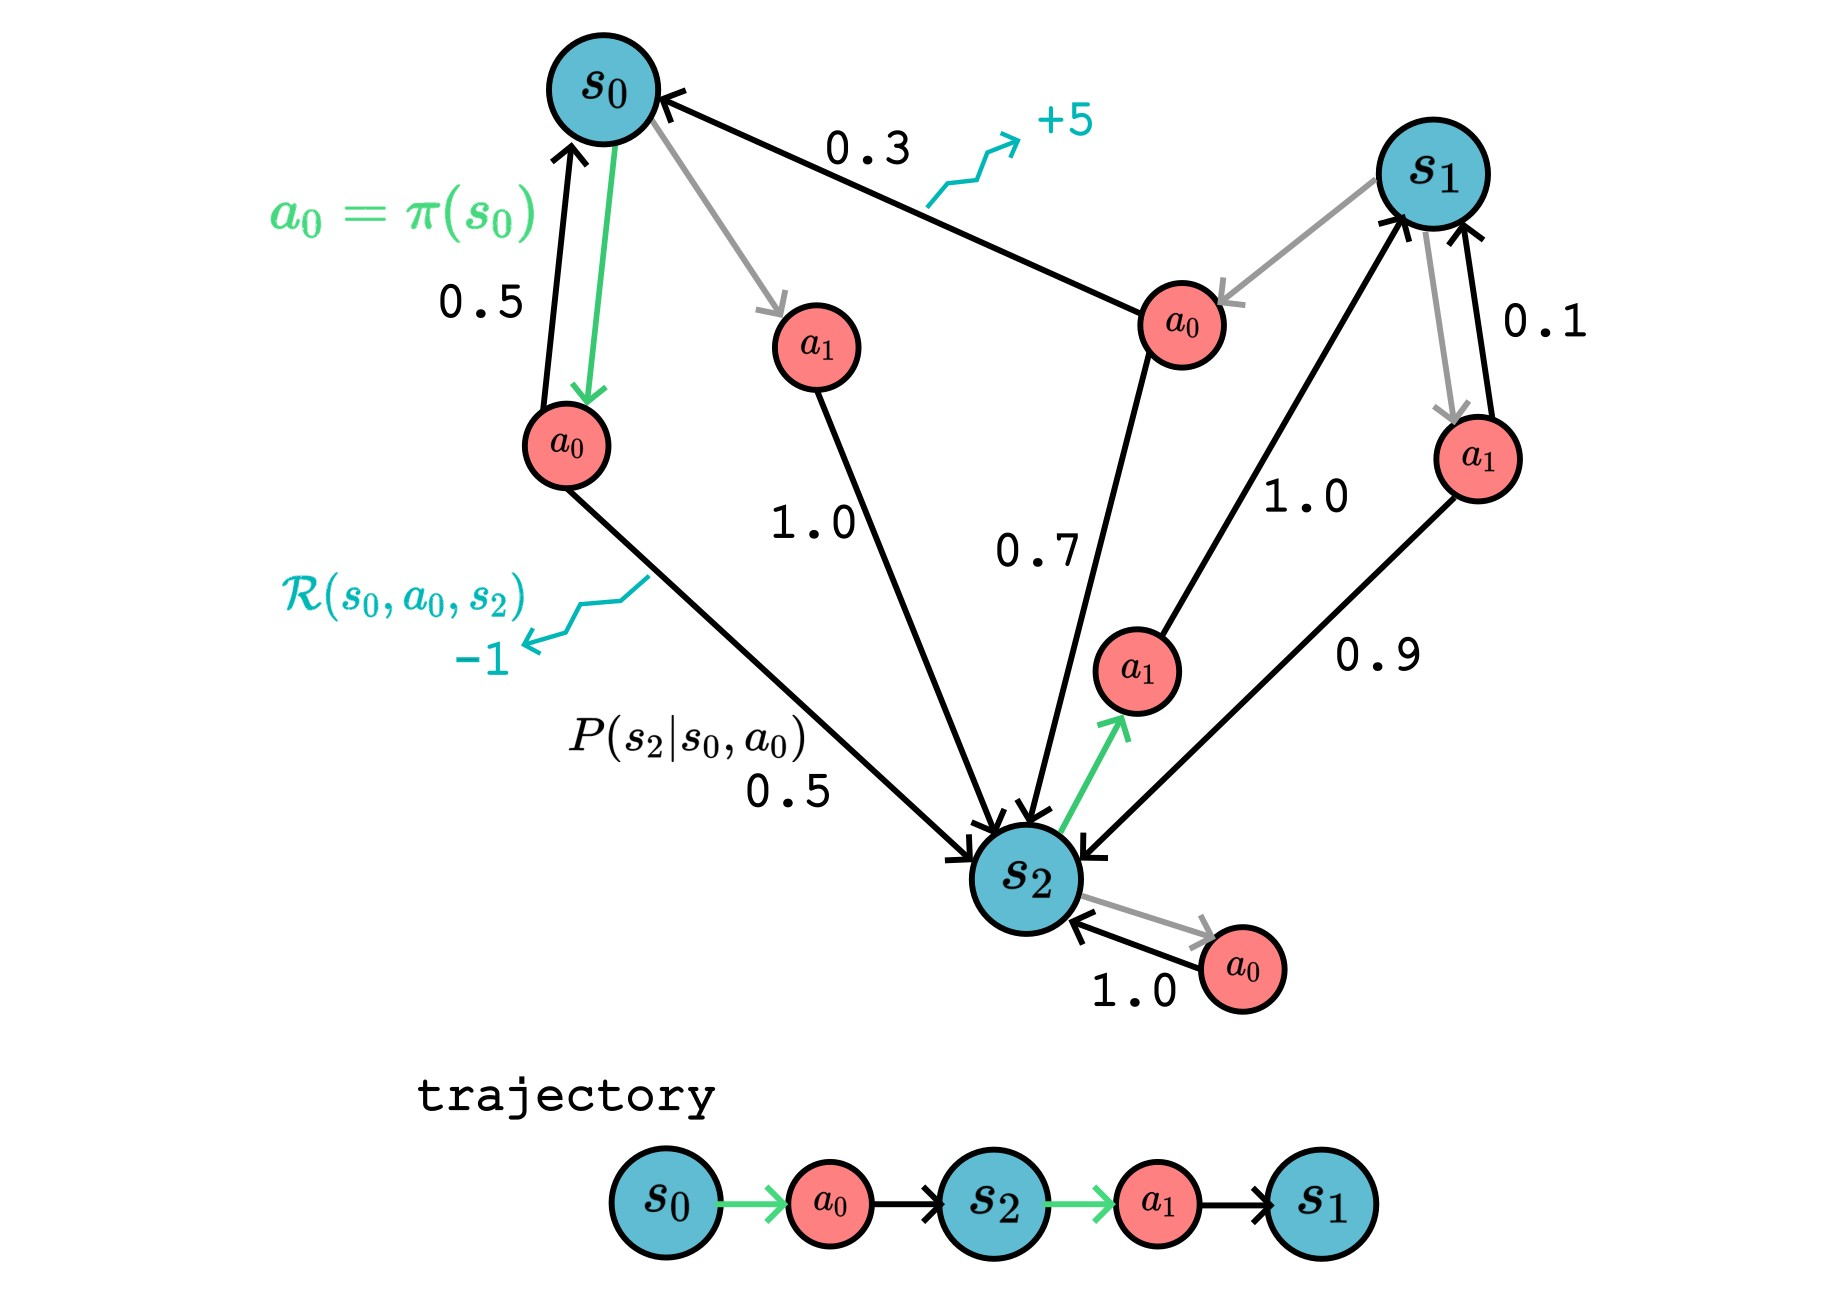
\includegraphics[width=1\linewidth]{Figures/mdp.jpg}
    \caption[Markov Decision Process]{\textbf{Markov Decision Process.} TODO}
    \label{fig:mdp}
\end{figure}


%Intuitively, the reinforcement learning (RL) loop depicted in Figure \ref{fig:rl_loop} can be understood as a trial-and-error process that induces an MDP. 

% For instance, if the states are represented by image frames from a simulator, the corresponding MDP would be described by \ref{}.

A \textbf{policy} $\pi \in \mathcal{P}(\mathcal{A})^\mathcal{S}$ describes the agent actions in a given state. A stochastic policy is a mapping from states to distributions over actions
\begin{equation}
    a_t \sim \pi(\cdot|s_t)
\end{equation}
, while a deterministic policy is a direct mapping from states to actions
\begin{equation}
a_t = \pi(s_t)    
\end{equation} 

\subsection{Trajectories, Return, and Value Functions}

The iterative interaction of an agent in the environment (see Figure \ref{fig:mdp}) is depicted in a \textbf{trajectory}\footnote{The trajectory, return and value functions explanations were based on \href{https://spinningup.openai.com/en/latest/spinningup/rl_intro.html}{OpenAI Spinning Up}} (also called rollout or \textbf{episode}), which is a sequence of states and actions.
$$\tau = (s_0, a_0, s_1, a_1, \dots )$$

where a \textbf{transition} is what happen between state $s_t$ and state $s_{t+1}$, in a deterministic transition as 
$$s_{t+1} = f(s_t, a_t)$$, 
or a stochastic transition $$s_{t+1} \sim P(\cdot | s_t, a_t)$$, where the action come from the policy.

The \textbf{reward} function $\mathcal{R}$ in the current work depends only on the current state and action taken, such that
$$r_t = \mathcal{R}(s_t,a_t)$$

The \textbf{return} $\mathcal{R}(\tau)$ is defined as the cumulative reward over a trajectory. It can be represented as a \textbf{finite-horizon undiscounted return}, which is the sum of rewards obtained within a fixed window of steps:
$$\mathcal{R}(\tau) = \sum_{t=0}^T r_t$$

, or as the \textbf{infinite-horizon discounted return}, which is the sum of all rewards ever obtained by the agent, but discounted by how far in the future they’re obtained. This formulation of return includes a discount factor $\gamma \in (0,1)$, which provide better theoretical convergence guarantees:

$$\mathcal{R}(\tau) = \sum_{t=0}^\infty \gamma^t r_t$$

In RL, any agent aims to obtain an optimal policy $\pi^\ast$ that maximizes the expected return when the agent acts according to it.

\begin{equation}
    \pi^\ast = \operatorname*{arg max}_\pi \mathop{\mathbb{E}}\limits_{\tau \sim \pi}\left[\mathcal{R}(\tau) \right]
\label{eq:rl_objective}
\end{equation}

To achieve this goal, in many cases such as with DQN (as we will discuss later), it is necessary to have a notion of the value of a state or state-action pair. The \textbf{value} is defined as the expected return when starting from that state or state-action pair and then following a particular policy indefinitely. Below are some key concepts related to \textbf{value functions} retrieved from \cite{SpinningUp2018}:

\begin{itemize}
    \item The \textbf{On-policy Value Function} gives the expected return if you start in state $s$ and always act according to policy $\pi$:
    \begin{equation}
    V^\pi(s) = \mathop{\mathbb E}_{\tau \sim \pi} \left[\mathcal{R}(\tau | s_0 = s)\right]
    \end{equation}
    \item The \textbf{On-Policy Action-Value Function}, $Q^{\pi}(s,a)$, which gives the expected return if you start in state $s$, take an arbitrary action $a$ (which may not have come from the policy), and then forever after act according to policy $\pi$:
    \begin{equation}
    Q^{\pi}(s,a) = \mathop{\mathbb E}_{\tau \sim \pi}\left[R(\tau)\left| s_0 = s, a_0 = a\right.\right]
    \end{equation}
    \item The \textbf{Optimal Value Function}, $V^*(s)$, which gives the expected return if you start in state $s$ and always act according to the optimal policy in the environment:
    \begin{equation}
    V^*(s) = \max_{\pi} \underE{\tau \sim \pi}{\mathcal{R}(\tau)\left| s_0 = s\right.}
    \end{equation}
    \item The \textbf{Optimal Action-Value Function}, $Q^*(s,a)$, which gives the expected return if you start in state s, take an arbitrary action a, and then forever after act according to the optimal policy in the environment:
    \begin{equation}
        Q^*(s,a) = \max_{\pi} \underE{\tau \sim \pi}{\mathcal{R}(\tau)\left| s_0 = s, a_0 = a\right.}
        \label{eq:q_optimal_value}
    \end{equation}


\end{itemize}

% \subsection{Value Iteration}
% \subsection{Q-Learning}



\subsection{Deep Q-Learning (DQN)}
\label{sec:dqn}
The Deep Q-Learning (DQN) \cite{mnih2013playing, mnih2015human} algorithm introduced a novel approach to train Q-learning algorithms using neural networks in high-dimensional, partially observable state spaces (e.g., raw pixels). It effectively addresses two important challenges in training deep neural networks for RL, such as highly-correlated states and non-stationary distribution issues.  To address both issues, DQN introduced a experience replay mechanism, which facilitates breaking temporal data correlations, leading to approximate independent and identically distributed (iid) data distributions.

%The RL is by nature a temporal sequential process, which produces highly-correlated states, and additionally; the data distribution evolves as the algorithm learns new behaviors, which is called a non-stationary distribution. From a supervised learning perspective, they made complicated the training because a supervised learning requires identical independent distributed data.

% NO image for experience replay (see Figure \ref{})
\textbf{Experience Replay} (ER) functions as a dataset with a \textbf{fixed capacity} $N$, storing tuples of experiences from the agent's interactions with the environment at different time steps during training, represented as
$$e_t = (s_t, a_t, r_t, s_{t+1}), \quad e_t \in \mathcal{E}$$

% In some scenarios, it is even possible to include a variable discount factor for each experience, such as $e_t = (s_t, a_t, r_t, \gamma_t, s_{t+1})$.

During training, mini-batches are randomly sampled from the experience replay to train a neural network $Q_\theta$, which is tasked with approximating the optimal state-action value function $Q^*$. In fact, DQN learning aims to estimate this optimal state-action value function, such that the optimal policy\footnote{Notice that by definition $Q^*(s,a)$ in Equation \ref{eq:q_optimal_value} represents the expected return for starting in state $s$, taking an arbitrary action $a$, and then following the optimal policy forever after. Therefore, by selecting the action with the maximum Q-value, we obtain the optimal policy that maximizes the expected return, same as the main RL goal in Equation \ref{eq:rl_objective}.} is

\begin{equation}
    \pi^*(s) = \arg \max_a Q^* (s,a)
    \label{eq:optinal_q_policy}
\end{equation}

To estimate the Q-value function, the DQN algorithm relies on a loss function derived from the Bellman equations \cite{sutton2018reinforcement}, which state that the value of a state is the reward you expect to receive from that state, plus the value of the subsequent state you transition to.
\begin{align*}
Q^*(s,a) &= \underE{s'\sim P(\cdot | s,a)}{r_t + \gamma \max_{a'} Q^*(s',a')}.
\end{align*}

As we aim to approximate $Q(s, a; \theta) \approx Q^*(s, a)$, a Q-network is trained to reduce the mean-square error in the Bellman equation by minimizing a sequence of loss function $L_i(\theta_i)$ that changes at each iteration $i$
\begin{align*}
    L_i (\theta_i) & = \underE{e_t \sim \mathcal{E}}{(y_i - Q(s_t, a_t; \theta_i))^2} \\
    & = \underE{(s_t, a_t, r_t, s_{t+1}) \sim \mathcal{E}}{(r_t + \gamma \max_{a'} Q(s_{t+1}, a'; \theta^-_{i}) - Q(s_t, a_t; \theta_i))^2} 
\end{align*}

where the optimal targets $r_t + \gamma \max_{a'} Q^*(s',a')$ are substituted with \textbf{approximated target values} for iteration $i$
\begin{equation}
    y_i = r_t + \gamma \max_{a'} Q(s_{t+1}, a'; \theta^-_{i})
\end{equation}

, and the gradients respect to the parameters $\theta_i$ are

\begin{equation}
    \nabla_{\theta_i} L(\theta_i) = \underE{(s_t, a_t, r_t, s_{t+1}) \sim \mathcal{E}}{ \delta_t \nabla_{\theta_i}Q(s_t, a_t; \theta_i)} 
\end{equation}

where the \textbf{temporal difference error} (or td-error) for the $e_i$ experience tuple corresponds to
\begin{equation}
    \delta_i = r_t + \gamma \max_{a'} Q(s_{t+1}, a'; \theta^-_{i}) - Q(s_t, a_t; \theta_i)
\end{equation}

Several important considerations should be taken into account when using this loss function in practice.

\begin{itemize}
    \item The parameters $\theta^-_{i}$ corresponds to a separated copy of the q-network parameters that is updated with $\theta_{i}$ every C gradient descent steps to stabilize the training.
    % \item Unlike supervised learning, the target depends on the parameters $\theta_{i-1}$, which change over time as the algorithm learns new behaviors.
    % \item The algorithm is \textit{model-free} because it does not require an explicit estimation of transitions distribution $P$ that govern the system.
    \item Although the algorithm approximates the greedy policy in Equation \ref{eq:optinal_q_policy}, it learns this strategy by using a behavioral \textbf{$\epsilon$-greedy policy}, which encourages exploration by taking a random action with probability $\epsilon$ during training 
    \begin{equation}
        \pi^\epsilon(a | s) = 
        \begin{cases} 
        a \sim \text{Uniform}(\mathcal{A}) & \text{with probability } \epsilon \\
        \arg\max_{a} Q(s, a; \theta) & \text{with probability } 1 - \epsilon
        \end{cases}
    \end{equation}
    
    Typically, this epsilon value is annealed over iterations to maintain a small value as learning approaches convergence.
    \item When learning from pixels, multiple frames $n$ are typically \textbf{stacked together} to represent a state in a preprocessing step. Additionally, the same action can be repeated over the $n$ stacked frames using a method called \textbf{skip frames} to reduce the training load. Thus, a state will be represented by $s_{t} = \phi(\{x_{t-n}, x_{t-(n-1)}, \cdots, x_{t}\})$, where the function $\phi$ stacks a window of $n$ frames (commonly $n=4$) while repeating the same action. For simplicity, we will refer to states in the algorithm and not the preprocessing function, but it is important to remind the reader that stacking and skip frames are used in a preprocessing step.
\end{itemize}

Algorithm \ref{algorithm:dqn} presents the pseudo-code for the DQN algorithm, modified slightly from the version in Mnih et al. \cite{mnih2013playing, mnih2015human} to run for a fixed total budget of $T$ (the total number of steps during the entire training), rather than running it per episode. This facilitates easier and fair comparisons with other extensions of the algorithm.

%Additionally, the algorithm show a per sample update procedure instead of the whole minibatch in order to make the comparison with prioritized alternatives clearlier, but the reader has to remember that in practice the gradients are calculated with vectorized procedures in the whole batch.



% \begin{algorithm}
% \caption{Deep Q-learning with Experience Replay (Mnih et al. \cite{mnih2013playing, mnih2015human})}
% \label{algorithm:dqn}
% \begin{algorithmic}[1]
% \State \textbf{Input:} minibatch $k$, step-size $\eta$, replay period $K$ and size $N$, budget $T$ (total steps).
% \State \textbf{Initialize} action-value function $Q$ with random weights $\theta$
% \State \textbf{Initialize} target action-value function $Q^-$ with weights $\theta^- = \theta$
% \State \textbf{Initialize} replay memory $\mathcal{D} = \emptyset$ with capacity $N$, $\Delta = 0$
% % \State Observe $s_0$ and choose $a_0 \sim \pi^\epsilon_\theta(s_0)$ 
% \For{$t = 1$ to $T$}
%     \State Observe $s_t$
%     \State Choose action $a_t \sim \pi^\epsilon_\theta(s_t)$
%     \State Execute action $a_t$ and observe $r_t$ and $s_{t+1}$
%     \State Store transition $(s_t, a_t, r_t, s_{t+1})$ in $\mathcal{D}$
%     \If{$t \equiv 0 \mod K$}
%         \For{$j = 1$ to $k$}
%             \State Sample transition $e_j \sim \text{Uniform}(\mathcal{D})$
%             \State Set $y_j = 
%             \begin{cases} 
%                 r_j & \text{for terminal } s_{j+1}\\
%                 r_j + \gamma \max_{a'} Q^-(s_{j+1}, a'; \theta^-) & \text{otherwise}
%             \end{cases}$
%             \State Compute TD-error $\delta_j = y_j - Q(s_j, a_j)$
%             \State Accumulate weight-change $\Delta \leftarrow \Delta + \delta_j \cdot \nabla_\theta Q(s_j, a_j)$
%         \EndFor
%         \State Update weights $\theta \leftarrow \theta + \eta \cdot \Delta$, reset $\Delta = 0$
%         \State Every C optimizing steps update $\theta^- \leftarrow \theta$
%     \EndIf
% \EndFor
% \end{algorithmic}
% \end{algorithm}

\begin{algorithm}[h]
\caption{Deep Q-learning with Experience Replay (Mnih et al. \cite{mnih2013playing, mnih2015human})}
\label{algorithm:dqn}
\begin{algorithmic}[1]
\State \textbf{Input:} minibatch $k$, step-size $\eta$, replay period $K$ and size $N$, budget $T$ (total steps).
\State \textbf{Initialize} action-value function $Q$ with random weights $\theta$
\State \textbf{Initialize} target action-value function $Q^-$ with weights $\theta^- = \theta$
\State \textbf{Initialize} replay memory $\mathcal{D} = \emptyset$ with capacity $N$ %$\Delta_{\{\xi, \omega\}} = 0$, $\Delta_\omega = 0$, $p_1 = 1$
% \State Observe $s_0$ and choose $a_0 \sim \pi^\epsilon_\theta(s_0)$ 
\For{$t = 1$ to $T$}
    \State Observe $s_t$
    \State Choose action $a_t \sim \pi^\epsilon_\theta(s_t)$
    \State Execute action $a_t$ and observe $r_t$ and $s_{t+1}$
    \State Store transition $(s_t, a_t, r_t, s_{t+1})$ in $\mathcal{D}$
        % \For{$j = 1$ to $k$}
        \State Sample minibatch $B \sim \text{Uniform}(\mathcal{D})$ of transitions $e_j$
        % \State Compute importance-sampling weight $w_j = \left( N \cdot P(j) \right)^{-\beta} / \max_i w_i$
        \State Set $y_j = 
        \begin{cases} 
            r_j & \text{for terminal } s_{j+1}\\
            r_j + \gamma \max_{a'} Q^-(s_{j+1}, a'; \theta^-) & \text{otherwise}
        \end{cases}$
        \State Compute TD-error $\delta_j = y_j - Q(s_{j}, a_{j}; \theta)$, and TD-loss $\mathcal{L}_{\text{TD}} = \delta_j^2 $
        \State Perform a gradient descent step on $\mathcal{L}_{\text{TD}}$
        % \State Update transition priority $p_j \leftarrow |\delta_j|$
        \State Every C optimizing steps update $\theta^- \leftarrow \theta$
\EndFor
\end{algorithmic}
\end{algorithm}

\subsection{Prioritized Experience Replay}
\label{sec:per}
Schaul et al. \cite{schaul2015prioritized} explored the limitations of the ER and discovered that a DQN algorithm revisits the same experience tuple an average of eight times, with not all revisits leading to significant improvements. As a result, they proposed Prioritized Experience Replay (PER), which non-uniformly samples experiences from the replay buffer based on a priority measure. While they left room for exploring other potential priority measures, they hypothesized that TD-error could serve as an indicator of expected learning progress. According to Schaul et al. \cite{schaul2015prioritized}, the \textbf{Expected Learning Progress} (ELP) is the idealised criterion to assign a priority value with the amount the RL agent can learn from a transition in its current state. By using TD-error as a priority measure, they aimed to more frequently replay experiences that are likely to result in those greater improvements.

Specifically, the sampling probability $P(i)$ of an experience tuple $e_i$ is defined as
\begin{equation}
    P(i) = \frac{p_i^\alpha}{\sum_k p_k^\alpha}
\end{equation}

where $\alpha$ controls the degree of prioritization, with $\alpha = 0$ the uniform case, and $p_i$ is the priority of an experience tuple $e_i$. Then, a \textbf{proportional prioritization}\footnote{An alternative \textbf{ranked-based prioritization}, defined as $p_i = \frac{1}{rank(i)}$, was also evaluated, where the $rank(i)$ represents the index of the experience in the buffer sorted according the TD-error $| \delta_i |$. This strategy employs a piece-wise linear function with $k$ segments to enhance sampling efficiency} assigns the priority as 
\begin{equation}
    p_i = | \delta_i | + \epsilon
\end{equation}

where $\epsilon$ is used to revised experiences even when td-error equal zero. This strategy uses a 'sum-tree' data structure to sample efficiently from a large experience buffer without depending on the buffer capacity $N$.

% \footnote{An additional \textbf{ranked-based prioritization} $p_i = \frac{1}{rank(i)}$ was evaluated, where the $rank(i)$ is the index of the experience in the buffer sorted according the TD-error $| \delta_i |$. This strategy utilizes a piece-wise linear function with $k$ segments of equal probability, allowing to sample a segment and then sampling uniformly from that segment.} 

The prioritized method, however, introduces a bias in the estimation of the Q-values. As the algorithm prioritize certain experiences over others, they will be sampled more frequently than what normally occur; skewing the distribution of experiences. This skewness does not correspond to the actual distribution of experiences encountered in the environment (the true distribution), leading to biased Q-value estimates. To address this issue, Schaul et al. \cite{schaul2015prioritized} introduced a \textbf{weighted Importance Sampling} \cite{mahmood2014weighted} to adjust the contribution of each sampled experience in the update step, compensating for the fact that some experiences were over-sampled (and therefore should be down-weighted) while others were under-sampled (and therefore should be up-weighted). The weight per experience is defined as
\begin{equation}
    w_i = \left(\frac{1}{N} \cdot \frac{1}{P(i)} \right)^\beta
\end{equation}

, where $N$ is the buffer capacity, and $\beta$ is an hyperparameter to adjust the importance sampling, which in practice is annealed from an initial value $\beta_0$ to $1$. Additionally, this weight is normalized by the maximal weight $\frac{1}{\max_k w_k}$ to stabilize the learning by reducing very large updates (only scaling downwards). Then, the weighted gradient is defined as
\begin{equation}
    \nabla_{\theta_i} L(\theta_i) = \underE{(s_t, a_t, r_t, s_{t+1}) \sim \mathcal{E}}{ w_i \delta_t \nabla_{\theta_i}Q(s_t, a_t; \theta_i)} 
\end{equation}

Algorithm \ref{algorithm:dqn_per} presents the pseudo-code for the DQN algorithm including the PER extension. It is important to note that, for practical reasons, priorities are updated only for the transitions in the current sampled mini-batch, as it would be computationally inefficient to update the entire replay buffer, especially when it is large. Additionally, new transitions added to the experience replay are assigned with a maximum priority to ensure that all experiences are sampled at least once.

% TODO:
% Domingo acabar background
% Lunes - Martes acabar State of the art
% Miercoles - Jueves - Viernes Metodologia
% Sabado Domingo Lunes Resultados y discusion
% Martes Miercoles Jueves Revision y mejorar graficas (5-7 acabado)
% 8 Ver si incluyo la prueba teorica
% Y aplicar a trabajos

\begin{algorithm}[h]
\caption{DQN with Prioritized Experience Replay (PER) (Schaul et al. \cite{schaul2015prioritized})}
\label{algorithm:dqn_per}
\begin{algorithmic}[1]
\State \textbf{Input:} minibatch $k$, step-size $\eta$, replay period $K$ and size $N$, exponents $\alpha$ and $\beta$, budget $T$ (total steps).
\State \textbf{Initialize} action-value function $Q$ with random weights $\theta$
\State \textbf{Initialize} target action-value function $Q^-$ with weights $\theta^- = \theta$
\State \textbf{Initialize} replay memory $\mathcal{D} = \emptyset$ with capacity $N$, $p_1 = 1$ (inital priority) %$\Delta_{\{\xi, \omega\}} = 0$, $\Delta_\omega = 0$, $p_1 = 1$
% \State Observe $s_0$ and choose $a_0 \sim \pi^\epsilon_\theta(s_0)$ 
\For{$t = 1$ to $T$}
    \State Observe $s_t$
    \State Choose action $a_t \sim \pi^\epsilon_\theta(s_t)$
    \State Execute action $a_t$ and observe $r_t$ and $s_{t+1}$
    \State Store transition $(s_t, a_t, r_t, s_{t+1})$ in $\mathcal{D}$ with maximal priority $p_t = \max_{i < t} p_i$
    \If{$t \equiv 0 \mod K$}
        % \For{$j = 1$ to $k$}
        \State Sample minibatch $B$ of transitions $e_j$ with probability $P(j) = \frac{p_j^\alpha}{\sum_i p_i^\alpha}$    
        \State Compute importance-sampling weight $w_j = \left( N \cdot P(j) \right)^{-\beta} / \max_i w_i$
        \State Set $y_j = 
        \begin{cases} 
            r_j & \text{for terminal } s_{j+1}\\
            r_j + \gamma \max_{a'} Q^-(s_{j+1}, a'; \theta^-) & \text{otherwise}
        \end{cases}$
        \State Compute TD-error $\delta_j = y_j - Q(s_{j}, a_{j}; \theta)$, and TD-loss $\mathcal{L}_{\text{TD}} = \delta_j^2 $
        \State Perform a gradient descent step on $\mathcal{L}_{\text{TD}}$, weighting the updates by $w_j$
        \State Update transition priority $p_j \leftarrow |\delta_j|$
        \State Every C optimizing steps update $\theta^- \leftarrow \theta$
    \EndIf
\EndFor
\end{algorithmic}
\end{algorithm}



\section{Bisimulation}
\label{sec:bisimulation_background}

Bisimulation, a concept of behavioral similarity, is central to this work. In the following sections, we will outline the key definitions of bisimulation that form the basis of our approach. For convenience, we reused the notation from \cite{castro2021mico} that is used interchangeable from now on. The next-state distribution for a given state-action pair $(s, a)$ is defined as,
$$P^a_s = P(\cdot|s, a) \in \mathcal{P(S)}$$, and the associated immediate reward 
$$r^a_s = r_t = \mathcal{R}(s,a)$$ 
Note not get confused with $P^a_s \neq P(s'|s, a)$, the former represents a distribution and the second one a probability value.

% \subsection{Preliminaries Concepts}

% \subsubsection{Equivalence Relation}

% \begin{definition}[Equivalence Relation]
% Let $X$ be a set. An equivalence relation on $X$ is a subset $R \subseteq X \times X$ that satisfies the following three properties:
% \begin{enumerate}
%     \item \textbf{Reflexivity}: For all $x \in X$, $(x,x) \in R$;
%     \item \textbf{Symmetry}: For all $x, y \in X$, if $(x,y) \in R$ then $(y,x) \in R$;
%     \item \textbf{Transitivity}: For all $x, y, z \in X$, if $(x,y) \in R$ and $(y,z) \in R$ then $(x,z) \in R$.
% \end{enumerate}
% \end{definition}

% In mathematics, an equivalence relation is a binary relation that is reflexive, symmetric and transitive. A simpler example is equality. 

% \begin{enumerate}
%     \item Any number $a$ is equal to itself (reflexive).
%     \item  If $a=b$, then $b=a$ (symmetric).
%     \item If $a=b$ and $b=c$, then $a=c$ (transitive). 
% \end{enumerate}

% \subsubsection{Equivalence Classes}

% \subsubsection{Metric and Pseudo-metrics}



\subsection{Bisimulation in a Markov Decision Process}
Initially introduced in the field of concurrency theory, \textbf{bisimulation} \cite{li2006towards, abate2024bisimulation, baier2008principles} is an equivalence relation between states of a transition system (e.g. MDP) that preserves the branching structure of the system, and which thus can simulate each other in a stepwise manner. Two states are bisimilar if they can simulate each other's behavior, thereby a bisimulation serves as a form of state abstraction that groups states $x, y \in \mathcal{S}$  that are 'behaviorally equivalent'. 


\begin{definition}[Bisimulation relation, Givan et al. \cite{givan2003equivalence}]
\label{def:bisimulation}
Given an MDP $M$, an equivalence relation $E$ between states is a \textbf{bisimulation relation} if, for all states $x, y \in \mathcal{S}$ that are equivalent under $E$ the following conditions hold:
% \begin{enumerate}
%     \item $\mathcal{R}\left(s_i, a\right) =\mathcal{R}\left(y, a\right) \quad \forall a \in \mathcal{A},$
%     \item $\mathcal{P}\left(G \mid s_i, a\right) =\mathcal{P}\left(G \mid y, a\right) \quad \forall a \in \mathcal{A}, \quad \forall G \in \mathcal{S}_B,$
% \end{enumerate}
% \begin{align}
% \label{eq:reward_equivalence}
% \mathcal{R}\left(s_i, a\right) & =\mathcal{R}\left(y, a\right) & & \forall a \in \mathcal{A}, \\
% \label{eq:transition_equivalence}
% \mathcal{P}\left(C \mid s_i, a\right) & =\mathcal{P}\left(C \mid y, a\right) & & \forall a \in \mathcal{A}, \quad \forall C \in \mathcal{S}_E,
% \end{align}
\begin{align}
\label{eq:reward_equivalence}
% \mathcal{R}\left(x, a\right) & =\mathcal{R}\left(y, a\right) & & \forall a \in \mathcal{A}, \\
r^a_x & = r^a_y \\
\label{eq:transition_equivalence}
P_x^a(C) & = P_y^a(C) & & \forall a \in \mathcal{A}, \quad \forall C \in \mathcal{S}_E,
% P\left(C \mid x, a\right) & = P\left(C \mid y, a\right) & & \forall a \in \mathcal{A}, \quad \forall C \in \mathcal{S}_E,
\end{align}

where $\mathcal{S}_E$ is the partition of $\mathcal{S}$ under the relation $E$, and $P_x^a(C) = \sum_{x' \in C} P_x^a(x')$.

%According to this concept, 
Two states $x, y \in S$ are \textbf{bisimilar} if there exists a bisimulation relation $E$ such that $(x, y) \in E$; consequently, their optimal value functions are equal, \(V^\ast(x) = V^\ast(y)\)\footnote{Note that the converse does not hold; that is, even if \(V^\ast(x) = V^\ast(y)\), it does not necessarily imply that the states $x$ and $y$ are bisimilar according to this definition}.

\end{definition}

The properties in Equations \ref{eq:reward_equivalence} and \ref{eq:transition_equivalence} are referred to as \textbf{Reward Equivalence} and \textbf{Transition Equivalence}, respectively. There can be various equivalence relations that satisfy these conditions, but in most cases, we are interested in the largest equivalence relation, denoted by $\sim$ \footnote{The smallest bisimulation relation is the identity relation, which is a trivial solution where each equivalence class contains only a single state.}.

Intuitively, a bisimulation of a transition system allows us to replace a complex system with a simpler system that has fewer states while still capturing the same behavior as the original.
%(see Figure \ref{}).

\subsection{On-policy bisimulation}

The strong behavioral guarantees of the aforementioned bisimulation relation can potentially hinder their applicability for RL algorithms. This is because they strictly require \textbf{exact action matching} between states, which can be highly challenging to achieve in complex environments (as it will be illustrated in detail later with an example in Section \ref{sec:motivating_example}). For example, there may be actions that do not lead to positive outcomes, but the equivalence conditions will still require proper matching between them. In other cases, even when states exhibit similar optimal values, $V^*(x) = V^*(y)$, they may not satisfy the equivalence properties.

%(see Figure \ref{}), even when states exhibit similar optimal values, $V^*(x) = V^*(y)$, they may not satisfy the equivalence properties.

Under these circumstances, Castro's work \cite{castro2020scalable} proposes an \textbf{on-policy bisimulation relation}, which, instead of looking to all actions matching, \textit{focus only on the current policy actions}. This approach aligns better with what RL algorithm does, where commonly is of interest to keep a behavioral current policy which is updated iteratively as the learning progress; allowing to focus over time only on the transitions of interest. %(not in transition that does not lead to large values).

\begin{definition}[On-policy Bisimulation Relation, Castro \cite{castro2020scalable}]
\label{def:on-policy-bisimulation}
Given an MDP $M$, an equivalence relation $E^\pi$ between states is a $\pi$-\textbf{bisimulation relation} if, for all states $x, y \in \mathcal{S}$ that are equivalent under $E^\pi$ the following conditions hold:
\begin{align}
\label{eq:on_policy_reward_equivalence}
r_{x}^\pi & = r_{y}^\pi
 \\
\label{eq:on_policy_transition_equivalence}
\mathcal{P}_{x}^\pi\left(C \right) & =\mathcal{P}_{y}^\pi\left(C\right) \quad \forall C \in \mathcal{S}_{E^\pi},
\end{align}

where $\mathcal{S}_{E^\pi}$ is the partition of $\mathcal{S}$ under the relation $E^\pi$, and

\begin{equation}
\begin{aligned}
\label{eq:on_policy_reward_transition}
r_x^\pi & :=\sum_a \pi(a \mid x) r_x^a \\
\forall C \in \mathcal{S}_{E^\pi}, \mathcal{P}_x^\pi(C) & :=\sum_a \pi(a \mid x) \sum_{x^{\prime} \in C} P_x^a(x^{\prime})
\end{aligned}
\end{equation}

%According to this concept, 
Two states $x, y \in S$ are $\pi$-\textbf{bisimilar} if there exists a $\pi$-bisimulation relation $E^\pi$ such that $(x, y) \in E^\pi$; consequently, their on-policy value functions are equal, \(V^\pi(x) = V^\pi(y)\). Denoting the largest bisimulation relation as $\sim_\pi$.
\end{definition}

Notice that both reward and transition equivalence now only account for one action $a$, which is the action sampled from the policy $\pi$. This action could come from an stochastic or deterministic policy. 


\subsection{On-policy Bisimulation metric}

The direct use of bisimulation relations is generally problematic because these relations are highly sensitive to infinitesimal variations in the reward function and environmental dynamics (transitions), which often arise from data-driven estimations. As a result, it is highly unlikely to exactly satisfy reward and transition equivalence in practice. \textbf{Bisimulation metrics} \cite{ferns2004metrics, ferns2011bisimulation, ferns2014bisimulation, castro2020scalable} have been proposed to address this issue and provide a smoother notion of similarity than that offered by strict equivalence relations. These metrics are defined within a pseudometric space\footnote{Notice a pseudometric has a weaker "identity of indiscernibles" axiom $x = y \implies d(x,y) = 0$, which permits cases where two states, $x$ and $y$, may be behavioral distinct yet still have a distance of 0. Please refer to Appendix \ref{append:metrics} for a details explanation about metrics.} on $\mathcal{S}$ 
\begin{equation}
\mathcal{M(S)}= \{d \in [0, \infty)^{\mathcal{S} \times \mathcal{S}} : d \text{ symmetric and satisfies the triangle inequality}\}
\end{equation}
, where a distance function \(d : \mathcal{S} \times \mathcal{S} \rightarrow \mathbb{R}_{\geq 0}\) quantifies the '\textbf{behavioral similarity}' between two states. Accordingly, it is said that a pseudometric $d \in \mathcal{M}$ induces an equivalence relation $E_d := \{(x, y)|d(x, y) = 0\}$. In other terms, any two states with distance 0 will be collapsed onto the same equivalence class.

In this context, Castro's work \cite{castro2020scalable} proposed an \textbf{on-policy bisimulation metric}, which induces the on-policy bisimulation equivalence relation mention before, specifically the largest one $\sim_\pi$.

\begin{definition}[On-policy Bisimulation metric, Castro \cite{castro2020scalable} - Theorem 2]
\label{def:on_policy_bisimulation_metric}
A $\pi$-bisimulation metric $d^\pi_\sim$ is the unique fixed-point of the operator $T^\pi_K : \mathcal{M(S)} \rightarrow \mathcal{M(S)}$, where 
\begin{equation}
    \label{eq:on_policy_bisim_metric}
    T^\pi_K(d)(x, y) = |r^\pi_x - r^\pi_y| + \gamma \mathcal{W}_d(P^\pi_x,P^\pi_y) 
\end{equation}
, where $\mathcal{W}_d$ corresponds to the Kantorovich distance (also known as Wasserstein distance) over the set of distributions $\mathcal{P}(\mathcal{S})$ with based distance $d$, where the minimal transport cost is taken over all the couplings (see Section \ref{sec:coupling_kantorovich}).
\end{definition}

Notice a $\pi$-bisimulation metric allow us to relate the behavioral distances with the value function under the current policy $\pi$, using the following theoretical guarantee.
\begin{definition}[Theorem 3, Castro \cite{castro2020scalable}]
 Given any two states $x, y \in \mathcal{S}$ in an MDP, $|V^\pi(x) - V^\pi(y)| \leq d^\pi_\sim(x, y)$.   
\end{definition}

The operator $T^\pi_K(d)$ is a contraction mapping, which works as standard operators in dynamic programming for reinforcement learning (e.g. value iteration \cite{sutton1988learning, sutton2018reinforcement}), which in an iterative recurrent process will eventually converge to a fixed point $d^\pi_\sim$ up to an accuracy $\delta$, where $T^\pi_K(d)$ maps effectively $\mathcal{M}(S)$ into itself, and the operator corresponds to the bisimulation metric, that is $T^\pi_K(d) = d^\sim : S \times S \rightarrow \mathbb{R}$. Then, let an initial estimate $d_0$, we have iterative recurrent updates as

$$d_0 \rightarrow T^\pi_1(d_0) = d_1 \rightarrow T^\pi_2(d_1) = d_2 \cdots \rightarrow d^\pi_\sim$$

\subsection{Couplings and Kantorovich}
\label{sec:coupling_kantorovich}

In probability theory, \textbf{Coupling} \cite{lindvall2002lectures} is a method that allows us to related two (possible unrelated) random variables $X, Y$ by constructing a new joint random variable $(W,Z)$, such that the marginal distributions corresponds to $X, Y$, that is
\begin{align}
    P(W = w) & = \sum_z P(W = w, Z = z) = P(X) \\
    P(Z = z) & = \sum_w P(W = w, Z = z) = P(Y)
\end{align}

This coupling allow us to compare $X$ and $Y$ through the behavior of the joint distribution $(W,Z)$. Notice that there can be different couplings from joint distributions that satisfy the marginal distribution conditions; but in most cases we are interested in analyzing joint distributions where $W$ and $Z$ are dependent.

The \textbf{Kantorovich (or Wasserstein) distance} \cite{villani2009optimal} is defined as the minimum cost required to transform one probability distribution into another, often conceptualized as transporting mass from one distribution to another. This distance is based on the concept of coupling, where the optimal coupling represents the most efficient way to pair elements from the two distributions in order to move mass between them. In other words, the minimal cost is determined by finding the optimal coupling that minimizes the expected transport cost. In the on-policy bisimulation metric\footnote{Notice bisimulation metric uses the 1-Wassertein metric not the general case d-Wassertein metric.} (see Equation \ref{eq:on_policy_bisim_metric}), it is
\begin{equation}
% W_d\left(\mu, \nu\right)=\min _{\substack{\left(X, Y\right) \\ X \sim \mu, Y \sim \nu}} \mathbb{E}\left[d\left(X, Y\right)\right]
W_d(P_{x}^\pi, P_{y}^\pi) = \inf_{\psi \in \Psi(P_{x}^\pi, P_{y}^\pi)} \mathbb{E}_{(x',y') \sim \psi} \left[ d(x', y') \right]
\end{equation}
where 
\begin{itemize}
    \item $\Psi(P_{x}^\pi, P_{y}^\pi)$ is the set of all possible couplings of the distributions $P_{x}^\pi$ and $P_{y}^\pi$,
    \item $\psi(x',y')$ is a joint distribution that defines a coupling of $P_{x}^\pi$ and $P_{y}^\pi$, and 
    \item $d(x',y')$ is the distance between $x'$ and $y'$.
\end{itemize}
% where $\mu, \nu \in \mathcal{P}(\mathcal{S})$, and the minimum is taken over all the couplings $(X,Y)$ with the prescribed marginals.

\subsection{Matching under Independent Couplings (MICO) metric}

%Although the on-policy bisimulation aligns more closely with the RL framework by better connecting with the dynamics of the environment with the online policy, it still faces challenges when computed at large scales. 
The on-policy bisimulation metric still faces challenges when computed at large scales, mainly because it requires the exact computation of the Kantorovich distance, which involves solving an optimal transport problem. This process can be computationally expensive, particularly in high-dimensional spaces.

Although the on-policy bisimulation can be computed via fixed-point iteration on the operator $T_K^\pi$, the \textbf{iterative cost is significant}. According to Castro et al. \cite{castro2021mico}, the overall practical cost of computing a bisimulation metric is $\tilde{O}(|\mathcal{S}|^5 |\mathcal{A} \text{log}(\epsilon)/\text{log}(\gamma)$, where $\epsilon$ is the tolerance and $\gamma$ is the discount factor rate. Most of this complexity is dominated by the calculation of the Kantorovich distances $W_d$, which account for approximately $|\mathcal{S}|^2 |\mathcal{A}|$ per calculation. This makes it impractical to compute the metric for high-dimensional state spaces. Additionally, computing the Kantorovich distances \textbf{requires knowledge of the transition distributions}, which are typically not readily available. As a result, other works have employed approximators for the operator under deterministic conditions \cite{castro2020scalable} or Gaussian assumptions \cite{zhang2020learning} to estimate these distributions.

To address the aforementioned issues, Castro et al. \cite{castro2021mico} introduced the \textbf{Matching under Independent Coupling (MICo) metric}, which employs the independent coupling to replace the Kantorovich distance. While this surrogate metric introduces a looser bound on convergence guarantees, it offers a more tractable alternative that still provides valuable insights into state similarity, even though it does not capture the exact Kantorovich distance. Furthermore, it is broadly applicable to both deterministic and stochastic environments.

\begin{definition} [MICo update operator, Castro et al. \cite{castro2021mico}]
\label{def:mico_operator}
Given $\pi \in \mathcal{P(A)}^{\mathcal{S}}$, the MICO update operator $T^\pi_M : \mathbb{R}^{\mathcal{S} \times \mathcal{S}} \rightarrow \mathbb{R}^{\mathcal{S} \times \mathcal{S}}$

\begin{equation}
\label{eq:mico_operator}
    T^\pi_M(U)(x, y) = |r^\pi_{x} - r^\pi_{y}| + \gamma \mathbb{E}_{x'\sim P_x^\pi, y'\sim P_y^\pi}\left[U(x',y') \right]
\end{equation}

for all $U: \mathcal{S} \times \mathcal{S} \rightarrow \mathbb{R}$, with $r_x^\pi =\sum_a \pi(a \mid x) r_x^a$ and $P_x^\pi =\sum_a \pi(a \mid x) P^a_x(\cdot) $ for all $x \in \mathcal{S}$, 
\end{definition}

In an independent coupling, both $x'$ and $y'$ are sampled independently from $P_x^\pi(x')$ and $P_y^\pi(y')$, respectively, with no attempt to optimize the joint distribution $\psi$ to minimize the expected distance $U$, and having $\psi(x',y') = P_x^\pi \cdot P_y^\pi$.

Similar to the on-policy bisimulation metric, the MICo operator $T^\pi_M$ is a contraction mapping and has a unique fixed point $U^\pi \in \mathbb{R}^{\mathcal{S} \times \mathcal{S}}$. An iterative recursive application of the operator will converge to that fixed point. Additionally, the MICo operator provides similar theoretical guarantees as other bisimulation metrics.
\begin{equation}
    | V^\pi(x) -V^\pi(y) | \leq U^\pi(x,y)
\end{equation}

\subsubsection{Diffuse Metric}

The MICo metric is not a standard metric; it is a \textbf{diffuse metric}.

\begin{definition} [Diffuse metric, Castro et al. \cite{castro2021mico}]
\label{def:diffuse_metric}
    Given a set $X$, a function $d : X \times X \rightarrow \mathbb{R}$ is a diffuse metric if the following axioms hold: (i) $d(x, y) \geq 0$ for any $x, y \in X$ ; (ii) $d(x, y) = d(y, x)$ for any $x, y \in X$ ; (iii) $d(x, y) \leq d(x, z) + d(y, z)$ $\forall x, y, z \in X$ .
\end{definition}

According to condition (i), in addition to being a pseudo-metric (like the on-policy bisimulation metric, which allows zero values for distinct states), a diffuse metric permits \textbf{self-distances greater than zero}.

Formally, the second term in the MICo operator (Equation \ref{eq:mico_operator}) coincides with the Lukaszyk-Kaminski distance \cite{lukaszyk2004new}:
\begin{equation}
    d_{LK}(d)(\nu, \mu) = \mathbb{E}_{X \sim \nu, Y \sim \mu}[d(X,Y)],
\end{equation}
which is itself a diffuse metric. Consequently, the MICo metric is also a diffuse metric, with a fixed point given by $U^\pi = |r^\pi_x - r^\pi_y | + d_{LK}(U^\pi)(P^\pi_x, P^\pi_y)$.

% Although it might initially seem counterintuitive to have self-distances greater than zero, this approach provides a more tractable alternative, especially in accounting for stochasticity in trajectories, particularly when the action space is continuous and policies are stochastic. In such scenarios, we may encounter broad trajectories with significant overlap, making it difficult to distinguish between them.

% In these cases, a notion of a diffuse distance is valuable for capturing this stochasticity. Specifically, the Lukaszyk-Kaminski distance measures the expected distance between random variables from two distributions without requiring a perfect match between points. This distance quantifies the "spread" between distributions rather than relying on exact point-to-point distances.

% By incorporating this term, the MICO metric shares characteristics with diffuse metrics by emphasizing expected similarities and overlaps in distributions, making it robust against variability and noise. It reflects similarities between distributions even when their underlying states do not match exactly, which is crucial in reinforcement learning scenarios where distributions of states overlap but are not identical, making exact state matching impractical.

Although it might initially seem counterintuitive for self-distances to be greater than zero, this approach offers a practical alternative, especially in scenarios where the policies are stochastic. In such cases, trajectories can overlap significantly, complicating the distinction between them.

The Lukaszyk-Kaminski distance $d_{LK}$ addresses this by measuring the expected distance between random variables from two distributions, focusing on the "spread" rather than exact point-to-point matches. This allows the MICO metric to capture expected similarities and overlaps between next-states distributions, making it robust against variability and noise. This is crucial in reinforcement learning, where state distributions often overlap without exact matching.

It is important to note that the notion of state self-distance serves as an indicator of the dispersion within the distribution \cite{castro2021mico}, having in general $U^\pi(x,x) > 0$ and $U^\pi(x,x) \neq U^\pi(y,y)$ for distinct states $x, y \in \mathcal{S}$. Nonetheless, $U^\pi(x,x) =0$ iff the policy $\pi$ is deterministic when evaluated at $x$.





% \section{Diffuse metric}

%\subsection{State Abstractions}











